\section{Beágyazott irányító rendszerek}
\vspace{5cm}
\subsection{Beágyazott irányító rendszerek típusai}

\subsection{Mikrovezérlő alapú rendszerek}

\subsection{Gyakran használt mikrovezérlő perifériák}

\subsubsection{AD Átalakítók}

\subsubsection{Timer és Capture perifériák}
Digitális irányító rendszerek esteében alapvető fontosságú a rendszer műküdését vezérlő úrajel jelenléte. Jelen fejezetben arra nem térünk ki, hogy ez az úrajel honnan származik, de úgy tekintjük, hogy jelen van a rendszerben, ismert a frekvenciája és a pontossága, amely segítségével lehetségessé válik idő és frekvenciamérési feladatok megvalósítása. 

\subsection{Beágyazott kommunikációs interfészek}

\subsection{Digitális kommunikációs vonalak felépítése}

Digitális eszközök közötti adatcserére az iparban szabványoks kommunikációs protokollokat, kommuinkációs formákat haszánlunk. Ezek rendkívül sokrétűek, az olvasó is találkozhat velük a mindennapjaiban, legyen szó egy FM rádióadásról, a GSM hálózatról, vagy egy Ethernet kapcsolatról. Ezek a kommunkációs eljárások különböző, standard rétegeket implementálnak, melyek akár fel is cserélhetőek egymás között. (Pl. TCP/IP alapú kapcsolat megvalósítható WiFi-n és vezetlekes Ethernet hálózaton is) Ilyen modellszerű leírást ad meg az Open Systems Interconnection model (OSI model) is.

\paragraph{Layer 1: Fizikai réteg}

A fizikai réteg azt határozza meg, hogy milyen fizikai közegen keresztül áramlik az információ az eszközök között. A fizikai réteg specifikálja, hogy vezetékes, vagy vezeték nélküli kapcsolatról van-e szó, az átvitt jelek sázmát, az elvárt feszültésgszinteket és időzítéseket, a moduláció módját. A fizikai réteg dönti el, hogy az adat mely irányba áramolhat, simplex (egy irányú), half duplex (időosztáyban két irányú), vagy full duplex (folyamatosan két irányú) kommunikációról beszélünk-e.

\paragraph{Layer 2: Adatkapcsolati réteg}

\begin{example}[\quad \large Zavarérzékenység]

A tanult soros kommunikációk fizikai rétegei közül melyek hasonlóak zavarérzékenység, ill. logikai működés szempontjából?


\end{example}

\subsubsection{I2C}

Az $I^2C$ (Inter-Integrated Circuit) egy szinkon, csomagkapcsolt soros kommunikációs forma, melyet 1982-ben definiált a Philips Semiconductor (ma NXP). Igen elterjed, általában nyomtatott áramkörön belül, a különböző digitális eszközök között használt kommunikációs forma. Több, kompatibilis változata is létezik, iylen pl. az SMBus.

Leggyakrabban külsö ADC-k, EEPROM-ok és egyéb Flash memóriák, digitális érzékelők,  vagy egyszerű kijelzők vezérlésésre alkalmazzák.

Az I2C kommunikáció fizikai rétege 2 vezetékeből áll, melyre a perifériák open-collectoros kimenetekkel csatlakoznak, emiatt a busz vezetékeit fel kell húzni tápfeszültésgre. A tápfeszültségre felhúzú ellenállás méretét a kommunikációs sebesség, illetve a buszon található eszközök kapcitív terhelése határozza meg. Ez azt is jelenti, hogy ha a buszon bármely ezköz lehúzza bármely vezetéket annak feszültsége 0 lesz. Ez a két vezeték az SCL, azaz az órajelet közvetítő vezeték, illetve az SDA azaz az adatot közvetítő vezeték. Mivel az I2C buszon jelek nem diferenciális jelvátvitellel közlekednek, hanem egy vezetéken, ami az elektronika közös referencia feszültségéhez (GND) képest változtatja az értékét, single-ended kommunikációs vonalnak nevezzük. I2C buszon a logikai magas szint a magas feszültségnek felel meg, míg a logikai alacsony szint, a kis feszültségnek. A MASTER egység az üzenetek kezdetét un. START bittel jelzi, amely nem más mint az SDA vezeték alacsony állapotba állítása az SCL vezeték lehúzása nélkül nélkül. A STOP bit hasonló logika mentén, az órajel fix magas állapota melletti SDA magasba állítást jelenti az üzenet végén.

\begin{figure}[htb]
\begingroup
\tikzset{}
 \centerline{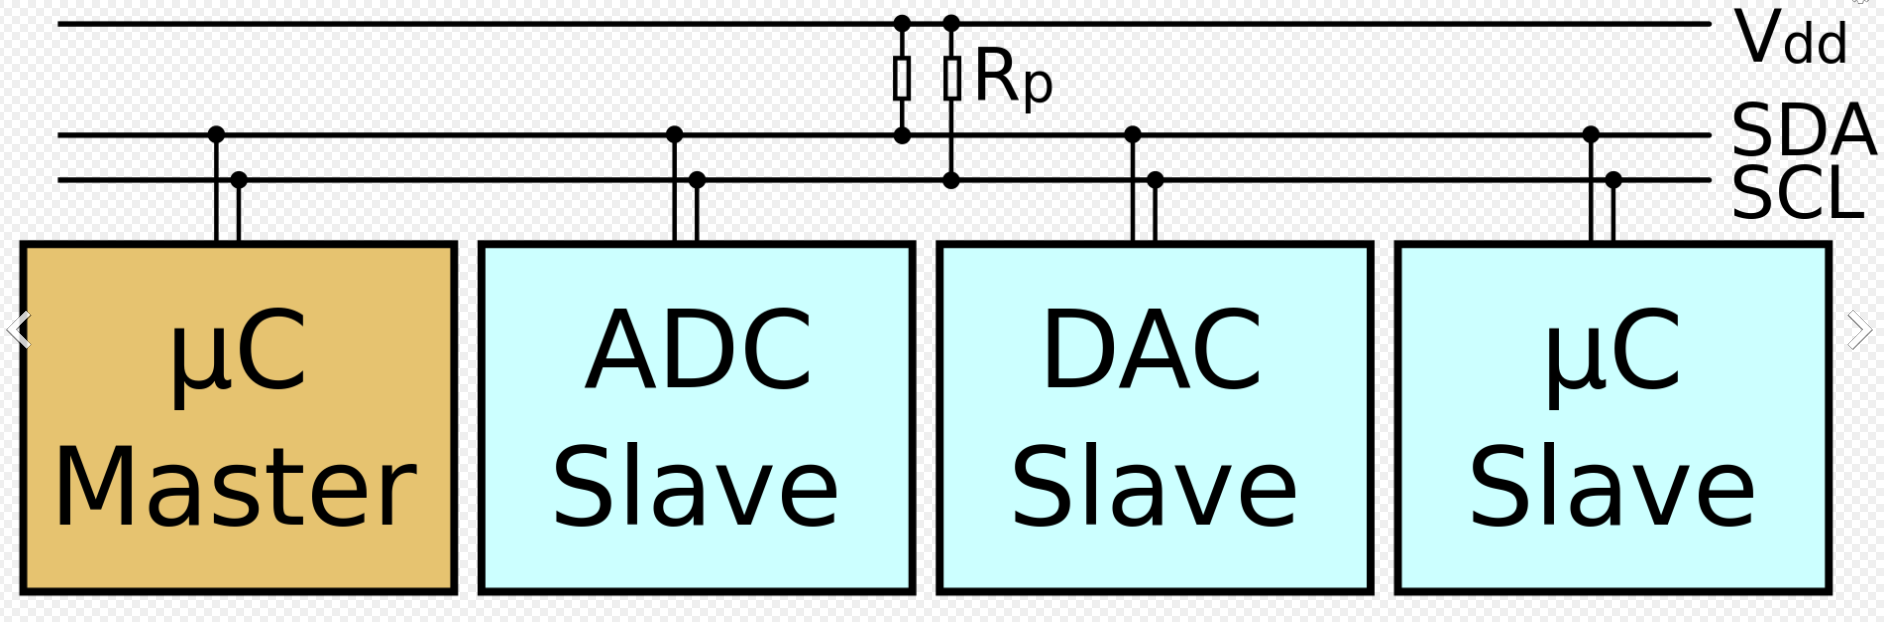
\includegraphics[width=0.6\columnwidth]{.//Figures/tmp/i2c_bus.png}}
 \endgroup
 \caption{I2C busz elrendezés}
 \label{fig:i2c_bus}
\end{figure}

A buszon két típusú eszköz található:
\begin{itemize}
    \item Master - ezen ezközök indítják a kommunikációt
    \item Slave - ezen eszközök reagálnak a kommunikációs kérdésekre
\end{itemize}

Egy buszon szerepelhet több master is, illetve a szerepeket akár dinamikusan is cserélhetik az eszközök, egyszerre azonban csak egyetlen eszköz adhat a buszon.

A buszon az eszközök alábbi üzemállapotokkal fordulhatnak elő:
\begin{itemize}
    \item master transmit
    \item master receive
    \item slave transmit
    \item slave receive
\end{itemize}

A buszon található különböző egységek megkülönböztetésére a cím szolgál. A master egység a START bit leadása után a MASTER elküldi a SLAVE egység 7 bites címét, majd ez után 1 bitben jelzi, ohgy írni (0), vagy olvasni (1) kíván az adott eszközbe/eszközből. Amennyiben a megcímzett SLAVE egység elérhető a buszon, így egy ACK bit kiadásával válaszol. A gyakorlatban ez az SDA vonal lehúzásást jeleni egy bit idejére.




\begin{example}[\quad \large I2C 1]

Ismertesse az I2C busz adatkapcsolati rétegét! Rajzoljon fel egy elrendezést 2 potenciális mester és 2 szolga résztvevővel! Vázolja fel a busz jeleit, ha a mester a 3 című eszközre egy 0 értékű és 255 értékű byte-ot ír és az eszköz képes a vételre!


\tcbline
\vspace{1mm}

\solution

\end{example}
\begin{example}[\quad \large I2C 2]

Ismertesse az I2C busz adatkapcsolati rétegét! Rajzoljon fel egy elrendezést 1 mester és 2 szolga résztvevővel! Vázolja fel a busz jeleit, ha a mester a 3 című eszközre egy 0 értékű byte-ot ír és az eszköz képes a vételre!


\tcbline
\vspace{1mm}

\solution

\end{example}
\begin{example}[\quad \large I2C 3]

Ismertesse az I2C busz adatkapcsolati rétegét! Rajzoljon fel egy elrendezést 1 mester és 2 szolga résztvevővel! Vázolja fel a busz jeleit, ha a mester a 127 című eszközre egy 0 értékű byte-ot ír és az eszköz képes a vételre!

\tcbline
\vspace{1mm}

\solution

\end{example}
\begin{example}[\quad \large I2C 4]

Ismertesse egy I2C buszos EEPROM egyetlen adatbájtja olvasásának fázisait.

\tcbline
\vspace{1mm}

\solution

\end{example}
\begin{example}[\quad \large I2C 5]

Rajzoljon fel egy elrendezést 1 mester és 2 szolga résztvevővel! Mi történik, ha a mester tévedésből két azonosra állított című eszközből olvas, ha az egyik eszközből olvasandó adat 0xaa, a másikból 0x55?

\tcbline
\vspace{1mm}

\solution

\end{example}


\subsubsection{SPI}

\begin{example}[\quad \large SPI 1]

Rajzoljon fel egy mestert és két szolgát tartalmazó rendszert! 

\tcbline
\vspace{1mm}

\solution

\end{example}
\begin{example}[\quad \large SPI 2]

Egy abszolút pozíció érzékelőt SSI interfészen illesztünk a folyamatirányító számítógéphez. Ismertesse a bekötéshez szükséges vezetékek szerepét! Melyik pillanatban érvényes pozíciót kapjak meg az irányító egység?

\tcbline
\vspace{1mm}

\solution

\end{example}
\begin{example}[\quad \large SPI 3]

Adja meg egy 4 bites adatok duplex átadásakor az SCLK, MOSI, MISO, CS (SL) jelek időfüggvényét!

\tcbline
\vspace{1mm}

\solution

\end{example}

\subsubsection{UART}

\begin{example}[\quad \large UART 1]

Rajzoljon fel egy 4 állomásos RS485-ös rendszert! 

\tcbline
\vspace{1mm}

\solution

\end{example}
\begin{example}[\quad \large UART 2]

Hasonlítsa össze az RS422 és az RS485 szabványokat!

\tcbline
\vspace{1mm}

\solution

\end{example}
\begin{example}[\quad \large UART 3]

Aszinkron soros kommunikáció alapszintű protokollja. Pl.: 7E2. 

\tcbline
\vspace{1mm}

\solution

\end{example}
\begin{example}[\quad \large UART 4]

Két processzor között aszinkron kommunikációt valósítunk meg. Megfelelnek-e a ±2,5\%-os pontosságú órajel-generátorok, ha a kommunikációs mód 8E1? Mikor lehet szükség egynél több stop bitre?

\tcbline
\vspace{1mm}

\solution

\end{example}
\begin{example}[\quad \large UART 5]

Rajzolja fel egy két részvevős RS485 rendszer vezetéke GND-hez képesti feszültségének időfüggvényét, amikor az egyik résztvevő 0x5A kódot küld 7O2 kommunikációs módban!

\tcbline
\vspace{1mm}

\solution

\end{example}
\begin{example}[\quad \large UART 6]

Rajzoljon fel egy 4 résztvevős RS485 szabvány szerinti kommunikációs rendszert! Mit érzékelnek a vevők, ha egyik részvevő sem ad?

\tcbline
\vspace{1mm}

\solution

\end{example}

\subsubsection{CAN}

\begin{example}[\quad \large CAN 1]

Mi a soros és a párhuzamos visszaverődés-mentesítés? Mikor melyiket célszerű alkalmazni?

\tcbline
\vspace{1mm}

\solution

\end{example}
\begin{example}[\quad \large CAN 2]

Egy CAN buszon két eszköz egyszerre kezd adni egy-egy standard ID-jű üzenetet. Az első eszköz üzenetének azonosítója 120, a másiké 64. Rajzolja fel az első eszköz TX és RX jelének első 12 bitjét!

\tcbline
\vspace{1mm}

\solution

\end{example}
\begin{example}[\quad \large CAN 3]

Egy CAN buszon két eszköz egyszerre kezd adni egy-egy standard ID-jű üzenetet. Az első eszköz üzenetének azonosítója 2047, a másiké 0. Rajzolja fel az első eszköz TX és RX jelének első 8 bitjét! Rajzoljon fel egy 4 résztvevős RS485 szabvány szerinti kommunikációs rendszert!

\tcbline
\vspace{1mm}

\solution

\end{example}
\begin{example}[\quad \large CAN 4]

CAN buszon az 1. állomás átviteli sebességét 500kBaudra állítottuk, a 2. állomás sebességét 1MBaud-ra. Mi lesz a 2. állomás TxD és RxD jele az első 10us-ban, ha az 1. állomás ID=3 azonosítójú üzenetet kezd el küldeni?

\tcbline
\vspace{1mm}

\solution

\end{example}
\begin{example}[\quad \large CAN 5]

Mit jelent a bit szintű arbitráció? A CAN üzenet melyik része az arbitrációs mező?

\tcbline
\vspace{1mm}

\solution

\end{example}
\begin{example}[\quad \large CAN 6]

Hány bites a DLC mező. Miért?

\tcbline
\vspace{1mm}

\solution

\end{example}
\begin{example}[\quad \large CAN 7]

Hány bites a standard ID? Mit jelent az, hogy a CAN üzenet-orientált?

\tcbline
\vspace{1mm}

\solution

\end{example}
\begin{example}[\quad \large CAN 8]

Ismertesse a CAN (A) üzenet felépítését! Hogyan változik meg a buszon mérhető jelsorozat, ha az egyik aktív ill. passzív vevő a CRC-t hibásnak érzékeli? 

\tcbline
\vspace{1mm}

\solution

\end{example}
\begin{example}[\quad \large CAN 9]

Mi az “error frame” és mikor adja egy résztvevő?

\tcbline
\vspace{1mm}

\solution

\end{example}
\begin{example}[\quad \large CAN 10]

Két processzor között CAN kommunikációt valósítunk meg. Megfelelnek-e a ±2,5\%-os pontosságú órajel-generátorok? 

\tcbline
\vspace{1mm}

\solution

\end{example}


\vspace{-1.5mm}
\newpage